\chapter{Solutions et solubilité}\label{ch:g6:solutions-and-solubility}

On ouvre une bouteille d'eau gazeuse~: un sifflement, et un flot de
minuscules bulles monte de nulle part. Une seconde plus tôt, l'eau
semblait parfaitement limpide, et pourtant un gaz y était dissous depuis
le début. Les solides se dissolvent, les liquides aussi, et les gaz
également --- mais jamais sans limite. Ce chapitre nomme les parties
d'une solution et mesure la quantité d'une substance qu'un liquide peut
contenir.

\begin{recall}
Un solide qui \omterm{def:g2:mixing-and-dissolving:dissolve}{se dissout} dans l'eau disparaît à la vue et laisse le
liquide limpide~; ce liquide limpide est une solution, et ce qui a été
dissous s'y trouve toujours (\cref{ch:g2:mixing-and-dissolving}). Une
solution est un \omterm{def:g6:pure-substances-and-mixtures:homogeneous}{mélange homogène} d'\omterm{def:g6:pure-substances-and-mixtures:species}{espèces chimiques}
(\cref{ch:g6:pure-substances-and-mixtures}). Faire évaporer l'eau permet
de récupérer le solide dissous (\cref{ch:g3:separating-mixtures}).
\end{recall}

\begin{omfigure}
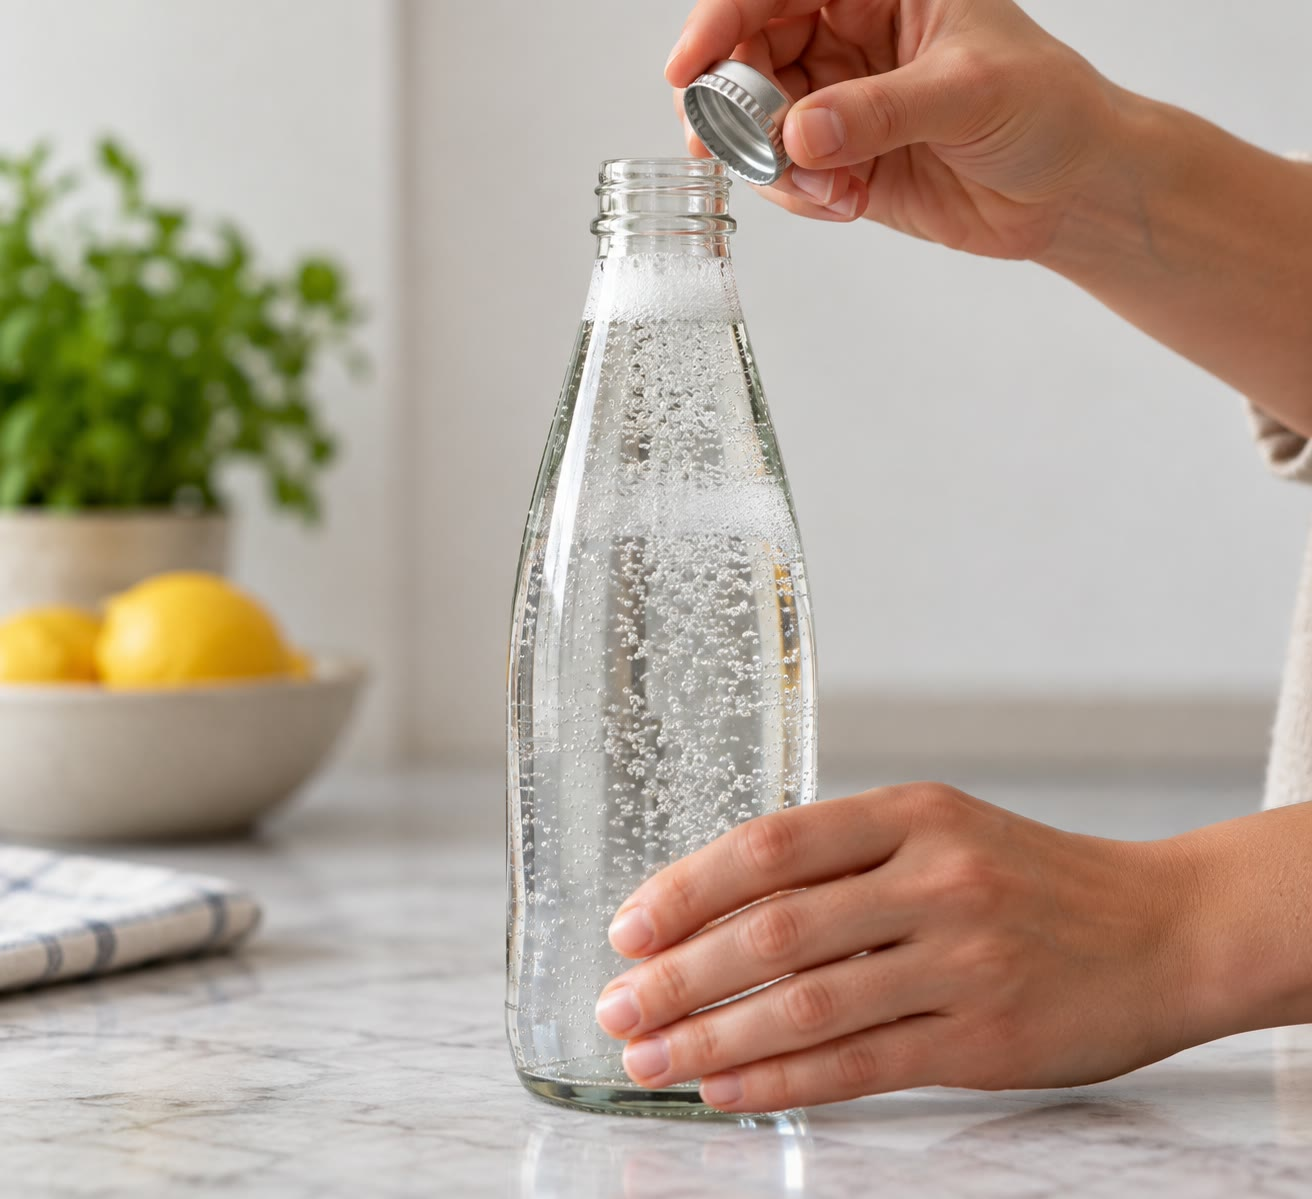
\includegraphics[width=0.5\linewidth]{images/book1/ai/g6-fizzy-water.jpg}

{\small On ouvre une bouteille d'eau gazeuse~: le gaz dissous ressort
sous forme de bulles.}
\end{omfigure}

\section{Soluté et solvant}

\begin{definition}[Soluté, solvant, solution aqueuse]\label{def:g6:solutions-and-solubility:solute}
Dans une solution, la substance qui \omterm{def:g2:mixing-and-dissolving:dissolve}{se dissout} est le
\emph{soluté}\index{solute@soluté}, et le liquide dans lequel elle \omterm{def:g2:mixing-and-dissolving:dissolve}{se dissout}
est le \emph{solvant}\index{solvant}. Quand le solvant est l'eau, la
solution est une \emph{solution aqueuse}\index{solution aqueuse}.
\end{definition}

\begin{example}[D'autres solvants que l'eau]\label{ex:g6:solutions-and-solubility:solvents}
L'eau est le \omterm{def:g6:solutions-and-solubility:solute}{solvant} le plus courant, mais pas le seul. Le vernis à
ongles ne \omterm{def:g2:mixing-and-dissolving:dissolve}{se dissout} pas dans l'eau~; il \omterm{def:g2:mixing-and-dissolving:dissolve}{se dissout} dans la propanone
(l'acétone), le \omterm{def:g6:solutions-and-solubility:solute}{solvant} du dissolvant pour vernis. La graisse et la
peinture à l'huile se dissolvent dans le white-spirit. Beaucoup de
médicaments sont dissous dans l'éthanol. Une solution peut avoir
plusieurs \omterm{def:g6:solutions-and-solubility:solute}{solutés}~: l'eau de mer contient du sel dissous et bien
d'autres substances.
\end{example}

\begin{safety}{\ghs{GHS02}\ghs{GHS07}}
% ledger: ghs:acetone
La propanone (acétone)~: liquide et vapeur très inflammables (GHS02)~;
elle irrite les yeux et sa vapeur peut provoquer somnolence ou vertiges
(GHS07). On l'utilise dans une pièce aérée, loin de toute flamme.
\end{safety}

\begin{proposition}[Les masses s'additionnent]\label{prop:g6:solutions-and-solubility:mass}
La masse d'une solution est la masse du \omterm{def:g6:solutions-and-solubility:solute}{solvant} plus la masse du \omterm{def:g6:solutions-and-solubility:solute}{soluté}
dissous~: rien ne se perd quand un solide \omterm{def:g2:mixing-and-dissolving:dissolve}{se dissout}, même si on ne le
voit plus.
\end{proposition}

\begin{omfigure}
\begin{tikzpicture}[font=\small, scale=1.15]
  \pic[transform shape] at (0,0) {balance};
  \pic[transform shape] at (0,0.8) {beaker={0.5}{omWater!80}};
  \node[anchor=north, align=center] at (0,-0.1) {\qty{100}{g} d'eau};
  \node at (1.85,1.3) {$+$};
  \pic[transform shape] at (3.5,0) {balance};
  \fill[white, draw=black!45] (3.0,0.8) rectangle (4.0,0.9);
  \fill[white, draw=black!45] (3.15,0.9) -- (3.85,0.9) -- (3.5,1.2) -- cycle;
  \node[anchor=north, align=center] at (3.5,-0.1) {\qty{10}{g} de sucre};
  \draw[->, thick, omProp] (4.9,1.2) -- (6.0,1.2) node[midway, above, text=black]
    {on remue};
  \pic[transform shape] at (7.4,0) {balance};
  \pic[transform shape] at (7.4,0.8) {beaker={0.52}{omWater!80}};
  \node[anchor=north, align=center] at (7.4,-0.1) {\qty{110}{g} d'eau sucrée};
\end{tikzpicture}

{\small Dissoudre \qty{10}{g} de sucre dans \qty{100}{g} d'eau donne
\qty{110}{g} de solution (la masse du bécher n'est pas comptée).}
\end{omfigure}

\section{Saturation et solubilité}

\begin{definition}[Solution saturée]\label{def:g6:solutions-and-solubility:saturated}
Une solution est une \emph{solution saturée}\index{solution saturee@solution saturée}
quand elle ne peut plus dissoudre davantage de son \omterm{def:g6:solutions-and-solubility:solute}{soluté}~: tout \omterm{def:g6:solutions-and-solubility:solute}{soluté}
ajouté reste au fond sans \omterm{def:g2:mixing-and-dissolving:dissolve}{se dissoudre}, même si l'on remue longtemps.
\end{definition}

\begin{definition}[Solubilité]\label{def:g6:solutions-and-solubility:solubility}
La \emph{solubilité}\index{solubilite@solubilité} d'un \omterm{def:g6:solutions-and-solubility:solute}{soluté} dans un \omterm{def:g6:solutions-and-solubility:solute}{solvant} est la
plus grande masse de \omterm{def:g6:solutions-and-solubility:solute}{soluté} qu'une quantité donnée de \omterm{def:g6:solutions-and-solubility:solute}{solvant} peut
dissoudre, à une température donnée. Pour un solide dans l'eau, on la
donne souvent en grammes par litre (ou par kilogramme) d'eau.
\end{definition}

\begin{proposition}[Quelques solubilités dans l'eau]\label{prop:g6:solutions-and-solubility:values}
% ledger: sol:NaCl, sol:sucrose, sol:CO2, sol:O2 (O2: 31 mL/L, 31/24.0 x 32 = 0.041 g/L at 20 C)
Les \omterm{def:g6:solutions-and-solubility:solubility}{solubilités} mesurées dans l'eau sont extrêmement différentes~:
\begin{center}
\small
\begin{tabular}{lll}
\hline
\omterm{def:g6:solutions-and-solubility:solute}{soluté} & \omterm{def:g6:solutions-and-solubility:solubility}{solubilité} dans l'eau & conditions \\
\hline
sucre (saccharose) & environ \qty{2000}{g} par litre d'eau & température ambiante \\
sel (chlorure de sodium) & \qty{360}{g} par kilogramme d'eau & \qty{25}{\celsius} \\
dioxyde de carbone & environ \qty{1.5}{g} par litre & \qty{25}{\celsius}, sous le gaz \\
oxygène & environ \qty{0.04}{g} par litre & \qty{20}{\celsius}, sous le gaz \\
sable, craie & pratiquement nulle & --- \\
\hline
\end{tabular}
\end{center}
Un litre d'eau peut dissoudre plus que sa propre masse de sucre, mais
pas même un demi-gramme d'oxygène.
\end{proposition}

\begin{method}[Tout va-t-il se dissoudre~?]\label{met:g6:solutions-and-solubility:will-it}
Pour savoir si une masse $m$ de \omterm{def:g6:solutions-and-solubility:solute}{soluté} \omterm{def:g2:mixing-and-dissolving:dissolve}{se dissout} complètement dans un
volume d'eau~:
\begin{enumerate}
  \item chercher la \omterm{def:g6:solutions-and-solubility:solubility}{solubilité} du \omterm{def:g6:solutions-and-solubility:solute}{soluté} (en g par litre d'eau)~;
  \item calculer la plus grande masse que ce volume d'eau peut
        dissoudre~;
  \item comparer avec $m$~: si $m$ est plus petite, tout \omterm{def:g2:mixing-and-dissolving:dissolve}{se dissout}~; si
        $m$ est plus grande, la solution est saturée et le reste demeure
        au fond.
\end{enumerate}
\end{method}

\begin{example}[Du sel dans un verre]\label{ex:g6:solutions-and-solubility:glass}
% ledger: sol:NaCl
\qty{50}{g} de sel peuvent-ils \omterm{def:g2:mixing-and-dissolving:dissolve}{se dissoudre} dans \qty{200}{mL} d'eau
(environ \qty{200}{g})~? Un kilogramme d'eau dissout au plus
\qty{360}{g} de sel, donc \qty{200}{g} d'eau en dissolvent au plus $360 \times
\frac{200}{1000} = \qty{72}{g}$. Comme $50 < 72$, tout le sel \omterm{def:g2:mixing-and-dissolving:dissolve}{se
dissout}.
\end{example}

\begin{omfigure}
\begin{tikzpicture}[font=\small, scale=1.15]
  \pic[transform shape] at (0,0) {beaker={0.6}{omWater!80}};
  \node[anchor=north, align=center] at (0,-0.15) {un peu de sel~:\\ tout est dissous};
  \pic[transform shape] at (3.2,0) {beaker={0.6}{omWater!80}};
  \node[anchor=north, align=center] at (3.2,-0.15) {plus de sel~:\\ tout juste saturée};
  \pic[transform shape] at (6.4,0) {beaker={0.6}{omWater!80}};
  \fill[black!12, draw=black!50] (5.7,0) -- (7.1,0) -- (6.9,0.2) -- (5.9,0.2) -- cycle;
  \foreach \x in {5.85,6.05,6.25,6.45,6.65,6.85} \fill[black!45] (\x,0.09) circle (0.03);
  \node[anchor=north, align=center] at (6.4,-0.15) {trop de sel~:\\ le reste ne se dissout pas};
\end{tikzpicture}

{\small On ajoute de plus en plus de sel à la même eau. Une fois la
\omterm{def:g6:solutions-and-solubility:saturated}{solution saturée}, le sel en trop reste au fond.}
\end{omfigure}

\begin{inthelab}[Saturer de l'eau en sel]
L'enseignant ajoute du sel à \qty{100}{mL} d'eau, une cuillerée à la
fois, en remuant bien après chacune. Les premières cuillerées
disparaissent~; puis une cuillerée ne \omterm{def:g2:mixing-and-dissolving:dissolve}{se dissout} plus entièrement et des
grains blancs restent au fond~: la solution est saturée. En pesant le
sel utilisé, on trouve qu'environ \qty{36}{g} se sont dissous.
\end{inthelab}

\section{Liquides miscibles et non miscibles}

\begin{definition}[Liquides miscibles et non miscibles]\label{def:g6:solutions-and-solubility:miscible}
Un liquide est \emph{miscible}\index{miscible} avec un autre quand,
mélangés, les deux donnent un seul liquide homogène. Il est
\emph{non miscible}\index{non miscible} avec lui quand les deux se
séparent en deux couches, la plus légère au-dessus.
\end{definition}

\begin{example}[L'eau et l'éthanol, l'eau et l'huile]\label{ex:g6:solutions-and-solubility:liquids}
L'eau et l'éthanol sont \omterm{def:g6:solutions-and-solubility:miscible}{miscibles}~: agités ensemble, ils donnent un seul
liquide limpide. L'eau et l'huile ne sont pas \omterm{def:g6:solutions-and-solubility:miscible}{miscibles}~: on a beau les
agiter fort, l'huile remonte et flotte sur l'eau en une couche séparée.
Dans un pot de vinaigrette, l'huile flotte au-dessus du vinaigre, qui
est surtout de l'eau.
\end{example}

\begin{omfigure}
\begin{tikzpicture}[font=\small, scale=1.3]
  \pic[transform shape] at (0,0) {testtube={0.6}{omWater!80}};
  \node[anchor=north, align=center] at (0,-0.15) {eau + éthanol~:\\ une couche};
  \pic[transform shape] at (3,0) {testtube={0.65}{yellow!55!orange!60}};
  \begin{scope}
    \clip (2.75,3) -- (2.75,0.25) arc[start angle=180, end angle=360, radius=0.25]
      -- (3.25,3) -- cycle;
    \fill[omWater!80] (2.7,0) rectangle (3.3,1.1);
  \end{scope}
  \draw[omGlass, line width=0.7pt] (2.75,3) -- (2.75,0.25) arc[start angle=180,
    end angle=360, radius=0.25] -- (3.25,3);
  \draw[<-, omProp, thick] (3.3,1.55) -- (4.1,1.75) node[right, text=black] {huile};
  \draw[<-, omProp, thick] (3.3,0.6) -- (4.1,0.6) node[right, text=black] {eau};
  \node[anchor=north, align=center] at (3,-0.15) {eau + huile~:\\ deux couches};
\end{tikzpicture}

{\small Des liquides \omterm{def:g6:solutions-and-solubility:miscible}{miscibles} donnent une couche~; des liquides \omterm{def:g6:solutions-and-solubility:miscible}{non
miscibles} en donnent deux.}
\end{omfigure}

\begin{omfigure}
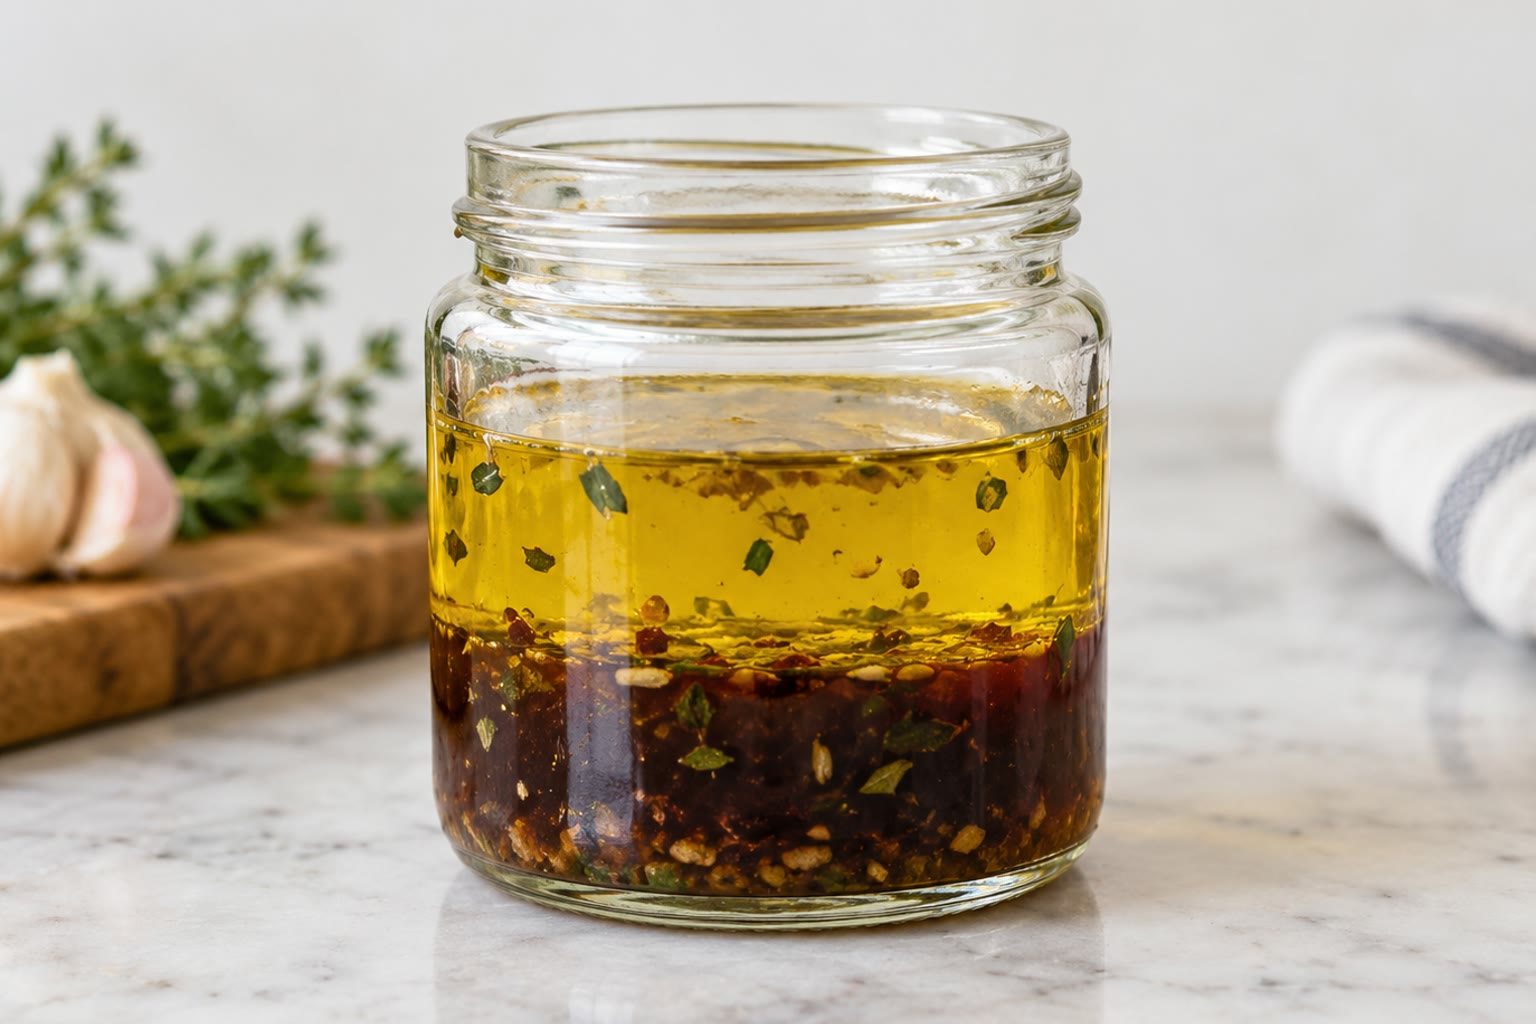
\includegraphics[width=0.45\linewidth]{images/book1/ai/g6-vinaigrette.jpg}

{\small La vinaigrette~: l'huile et le vinaigre ne sont pas \omterm{def:g6:solutions-and-solubility:miscible}{miscibles}.}
\end{omfigure}

\section{Les gaz se dissolvent aussi}

\begin{proposition}[Les gaz dissous]\label{prop:g6:solutions-and-solubility:gases}
Les gaz se dissolvent dans l'eau, un peu. On fabrique les boissons
gazeuses en y dissolvant du dioxyde de carbone sous pression, dans une
bouteille fermée~; quand on ouvre la bouteille, une partie du gaz
ressort sous forme de bulles. L'eau au contact de l'\omterm{def:g4:air-a-mixture-of-gases:air}{air} contient de
l'oxygène dissous, que les poissons prélèvent par leurs branchies. Un
gaz \omterm{def:g2:mixing-and-dissolving:dissolve}{se dissout} moins dans l'eau chaude que dans l'eau froide~: une
boisson gazeuse tiède perd plus vite ses bulles.
\end{proposition}

\begin{example}[Les océans et le dioxyde de carbone]\label{ex:g6:solutions-and-solubility:oceans}
Les océans sont au contact de l'\omterm{def:g4:air-a-mixture-of-gases:air}{air} sur les deux tiers de la surface de
la Terre. Le dioxyde de carbone de l'\omterm{def:g4:air-a-mixture-of-gases:air}{air} s'y dissout~: les océans
absorbent ainsi une partie du dioxyde de carbone que les humains
rejettent dans l'\omterm{def:g4:air-a-mixture-of-gases:air}{air}.
\end{example}

\begin{omfigure}
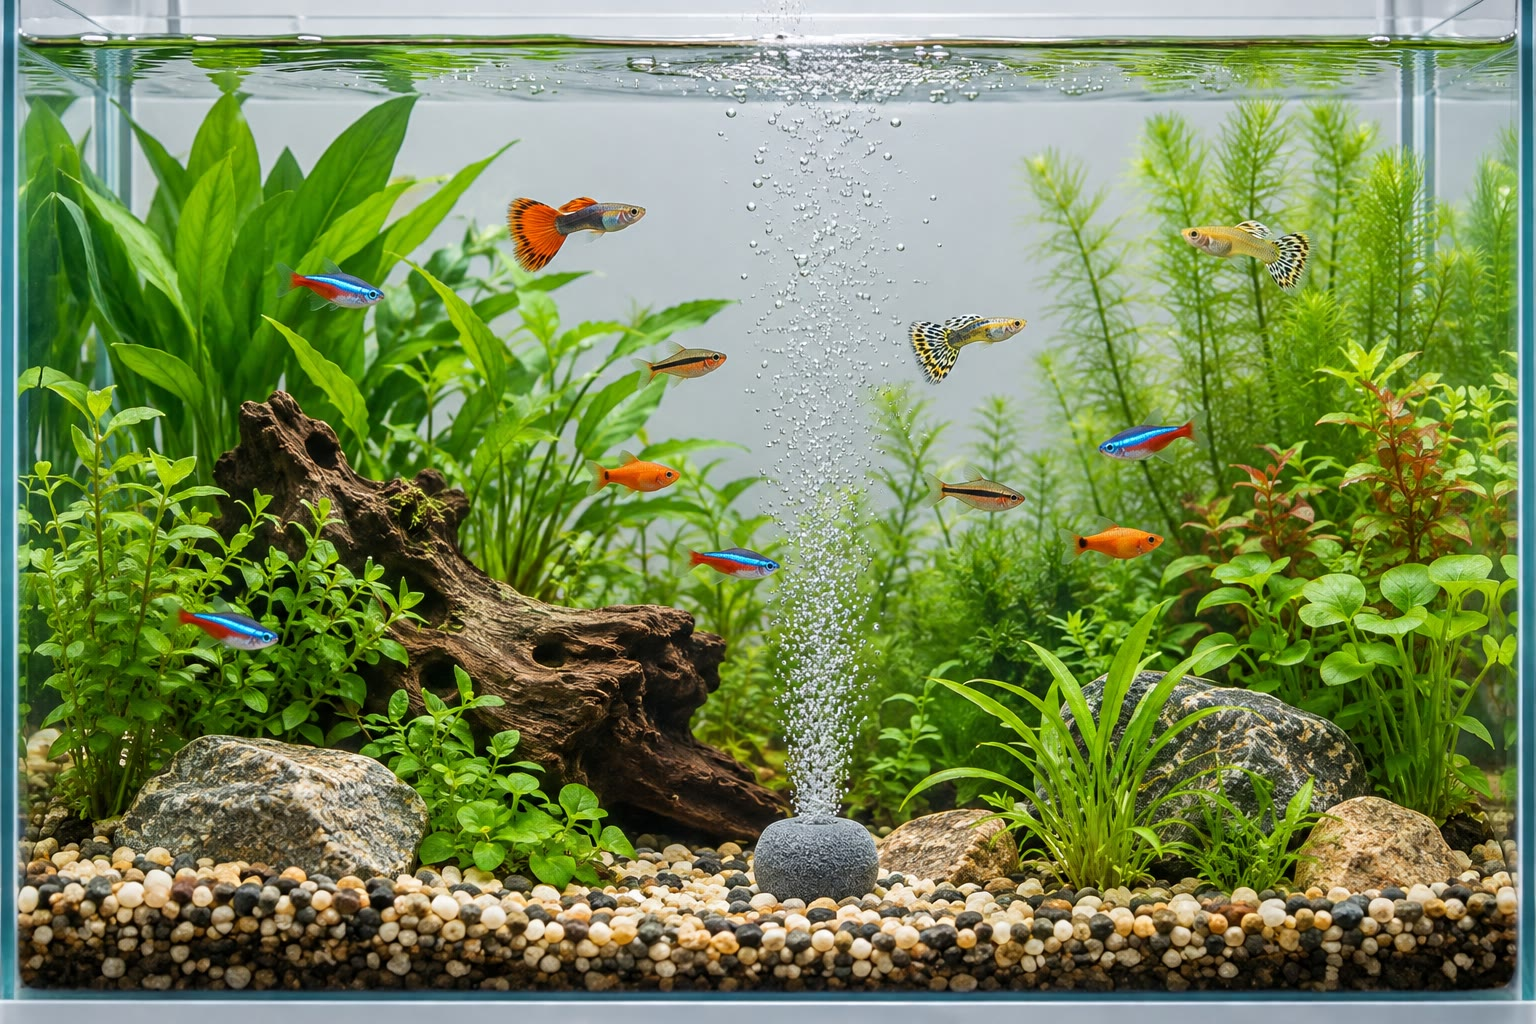
\includegraphics[width=0.5\linewidth]{images/book1/ai/g6-fish-tank.jpg}

{\small Un aquarium~: les bulles d'\omterm{def:g4:air-a-mixture-of-gases:air}{air} maintiennent dans l'eau de
l'oxygène dissous pour les poissons.}
\end{omfigure}

\section{Exercices}

\begin{exercise}[$\star$]\label{exo:g6:solutions-and-solubility:1}
Dans l'eau sucrée, nomme le \omterm{def:g6:solutions-and-solubility:solute}{soluté} et le \omterm{def:g6:solutions-and-solubility:solute}{solvant}. Est-ce une \omterm{def:g6:solutions-and-solubility:solute}{solution
aqueuse}~?
\end{exercise}

\begin{exercise}[$\star$]\label{exo:g6:solutions-and-solubility:2}
Qu'est-ce qu'une \omterm{def:g6:solutions-and-solubility:saturated}{solution saturée}~? Comment peut-on voir qu'une solution
est saturée~?
\end{exercise}

\begin{exercise}[$\star$]\label{exo:g6:solutions-and-solubility:3}
On dissout \qty{20}{g} de sel dans \qty{250}{g} d'eau. Quelle est la
masse de la solution~?
\end{exercise}

\begin{exercise}[$\star$]\label{exo:g6:solutions-and-solubility:4}
\omterm{def:g6:solutions-and-solubility:miscible}{Miscible} ou \omterm{def:g6:solutions-and-solubility:miscible}{non miscible} avec l'eau~: l'éthanol, l'huile de cuisine, le
vinaigre~?
\end{exercise}

\begin{exercise}[$\star$]\label{exo:g6:solutions-and-solubility:5}
Nomme le \omterm{def:g6:solutions-and-solubility:solute}{solvant} du dissolvant pour vernis à ongles et donne la
signification de ses deux pictogrammes.
\end{exercise}

\begin{exercise}[$\star\star$]\label{exo:g6:solutions-and-solubility:6}
À l'aide de la \omterm{def:g6:solutions-and-solubility:solubility}{solubilité} du sel, trouve la plus grande masse de sel que
\qty{500}{g} d'eau peuvent dissoudre à \qty{25}{\celsius}.
\end{exercise}

\begin{exercise}[$\star\star$]\label{exo:g6:solutions-and-solubility:7}
On remue \qty{80}{g} de sel dans \qty{200}{g} d'eau à
\qty{25}{\celsius}. Tout se dissout-il~? Sinon, quelle masse reste au
fond~?
\end{exercise}

\begin{exercise}[$\star\star$]\label{exo:g6:solutions-and-solubility:8}
On dissout \qty{25}{g} de sucre dans \qty{225}{g} d'eau. Quel
pourcentage de la masse de la solution est du sucre~?
\end{exercise}

\begin{exercise}[$\star\star$]\label{exo:g6:solutions-and-solubility:9}
Regarde la figure des trois béchers d'eau salée. Dans quel bécher
pourrait-on encore dissoudre du sel~?
\end{exercise}

\begin{exercise}[$\star\star$]\label{exo:g6:solutions-and-solubility:10}
Pourquoi une bouteille d'eau gazeuse pétille-t-elle quand on l'ouvre, et
pas avant~?
\end{exercise}

\begin{exercise}[$\star\star\star$]\label{exo:g6:solutions-and-solubility:11}
Un litre d'eau peut dissoudre environ \qty{2000}{g} de sucre, mais
seulement environ \qty{0.04}{g} d'oxygène. Combien de fois plus de sucre
que d'oxygène cela fait-il~?
\end{exercise}

\begin{exercise}[$\star\star\star$]\label{exo:g6:solutions-and-solubility:12}
En été, l'eau d'un étang se réchauffe et les poissons montent à la
surface pour avaler de l'\omterm{def:g4:air-a-mixture-of-gases:air}{air}. Explique pourquoi à l'aide de ce chapitre.
\end{exercise}

\section{Problème~: la saumure du fromager}

\begin{problem}[{Problème du week-end --- un bain d'eau saturée en sel
pour les fromages, et ce que la chaleur de l'été lui fait}]
\label{pb:g6:solutions-and-solubility:1}
% ledger: sol:NaCl (360 g per kg of water; 1 L of water taken as 1 kg)
Beaucoup de fromages trempent quelques heures dans un bain de saumure~:
de l'eau saturée en sel. Un fromager remplit une cuve de \qty{20}{L}
d'eau (\qty{20}{kg}) et ajoute du sel jusqu'à ce qu'il en reste au fond
sans \omterm{def:g2:mixing-and-dissolving:dissolve}{se dissoudre}. On prend pour \omterm{def:g6:solutions-and-solubility:solubility}{solubilité} du sel \qty{360}{g} par
kilogramme d'eau.

\medskip
\noindent\textbf{Partie I --- Le vocabulaire.}
\begin{enumerate}
  \item Dans la saumure, quel est le \omterm{def:g6:solutions-and-solubility:solute}{soluté} et quel est le \omterm{def:g6:solutions-and-solubility:solute}{solvant}~?
  \item Que signifie «~saturée~» pour la saumure~?
  \item Pourquoi le fromager ajoute-t-il du sel jusqu'à ce qu'il en reste
        un peu au fond~?
\end{enumerate}

\medskip
\noindent\textbf{Partie II --- Préparer la saumure.}
\begin{enumerate}[resume]
  \item Quelle masse de sel \omterm{def:g2:mixing-and-dissolving:dissolve}{se dissout} dans les \qty{20}{kg} d'eau~?
  \item Quelle est la masse de la saumure (sans le sel non dissous)~?
  \item Quel pourcentage de la masse de la saumure est du sel~? Arrondis
        à l'unité.
  \item Un jour, on n'ajoute que \qty{5}{kg} de sel. La saumure est-elle
        saturée~? Combien de sel pourrait-elle encore dissoudre~?
\end{enumerate}

\medskip
\noindent\textbf{Partie III --- Un été chaud.}
Pendant une semaine chaude, \qty{5}{L} (\qty{5}{kg}) d'eau s'évaporent
de la saumure saturée de la partie II, sans perte de sel.
\begin{enumerate}[resume]
  \item Combien d'eau reste-t-il dans la cuve~?
  \item Quelle masse de sel cette eau peut-elle encore garder dissoute~?
  \item Que devient le sel que l'eau restante ne peut plus contenir~?
  \item Comment le fromager peut-il voir, en regardant, que cela s'est
        produit~?
  \item Calcule la masse de sel qui a cristallisé au fond de la cuve.
\end{enumerate}
\end{problem}
